\documentclass[10pt,a4paper]{article}
\usepackage[margin=18mm]{geometry}
\usepackage[T1]{fontenc}
\usepackage{lmodern,graphicx,booktabs,amsmath,amssymb,xcolor}
\usepackage[hidelinks]{hyperref}
\setlength{\parindent}{0pt}
\setlength{\parskip}{6pt}
\begin{document}
{\Large\bfseries Integral C7 cover gluing: a bounded negative}\par
23 November 2026 \quad Native correctness; unsigned [pcc:unverified]

\textbf{Outcome.} None of the 144 mixed-kernel maps in the frozen CM19
catalogue is integral under both remaining cover-gluing signs. The 12
compatible maps are all twice automorphisms. This identifies a concrete
obstruction: using this catalogue without determining the actual sign
does not construct a nontrivial Jacobian endomorphism.

\begin{center}
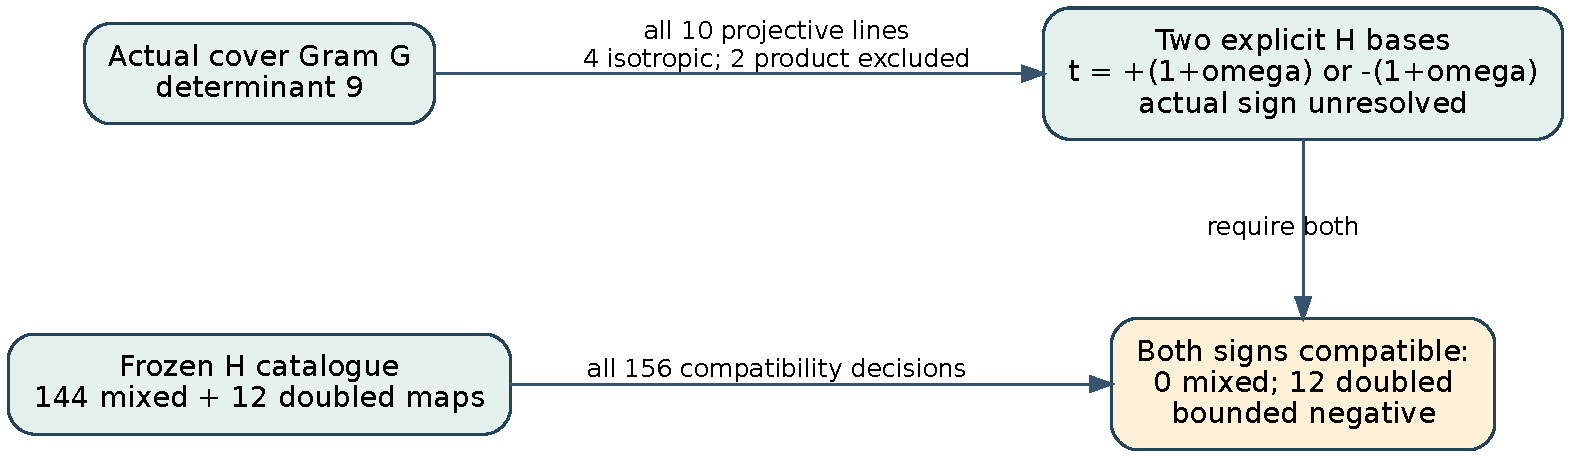
\includegraphics[width=\linewidth,height=64mm,keepaspectratio]{gluing.pdf}
\end{center}

\textbf{Actual correspondence basis.} The preceding qualified C7 covers
give $G=\left(\begin{smallmatrix}2&-1&0\\-1&2&0\\0&0&3\end{smallmatrix}\right)$.
For $\mathcal O=\mathbb Z[\omega]$, $\omega^2-\omega+5=0$, its
discriminant module is $(\mathcal O/3)^2$ with Hermitian numerator
$\operatorname{diag}(2,1)$. Among all ten projective lines over
$\mathbb F_9$, four are isotropic: $t=\pm1,\pm(1+\omega)$.
The first pair yields norm-one product polarizations, excluded by
Jacobian indecomposability. The other pair has explicit H-isometries:
\[
 T_+=\begin{pmatrix}1&1&0\\-(1+\omega)&0&1\\2-\omega&0&1\end{pmatrix},
 \quad T_-=T_+\operatorname{diag}(1,1,-1),
 \quad T_\pm^\dagger H T_\pm=G.
\]
Their determinants are $3,-3$. The interpretation uses the stated
ordinary-module/polarization dictionary and standard Jacobian
indecomposability; neither dependency is newly formally proved here.

\textbf{Complete fixed-family filter.} Parse all original 156 matrices,
checking their coefficients, identities, determinant norms and inherited
classes. For $A_0=\operatorname{adj}(T_+) S T_+$, require every
coefficient of $T_+ D A_0 D\operatorname{adj}(T_+)$ to be divisible
by nine. This is the exact second-sign integrality test. Every decision
and all 12 accepted numerator/twin matrices are retained.

\begin{center}
\begin{tabular}{lrr}
\toprule
Frozen class & Inputs & Both signs integral\\
\midrule
Mixed $[1,1,2,2,4,4]$ &144&0\\
Twice automorphisms $[2,2,2,2,2,2]$ &12&12\\
\bottomrule
\end{tabular}
\end{center}

Unsigned data 186804. All seven strict B phases exit zero, guards unchanged.
No prior vector grid, short-vector or similitude enumeration was rerun.
[pcc:unverified]
\newpage
{\Large\bfseries Controls, limits and the next geometric certificate}\par

\textbf{Controls distinguish more than counts.} Changing the Hermitian
form diagonal still gives four isotropic lines, but all four fail
integrality against the actual $G$. A real bridge-entry mutation fails
the full Gram identity, then pristine restores. Actual $2I$ is compatible;
a changed coefficient fails its actual H-similitude identity.

\textbf{What the negative establishes.} It covers this complete frozen
156-map family under the two explicit cover-basis identifications.
It excludes a sign-independent mixed map by this route. It does not
exclude mixed maps after determining the actual sign, different targets,
higher multipliers or other bases. The conditional selected 1331-point
EC-action branch did not execute and supplies no validated result.

\textbf{Execution and custody.} Frozen source
\texttt{fac647db}; all 31 complete inputs read back before execution.
Rust 1.99.1, warnings denied, overflow/debug assertions, one worker,
120s/2GiB per phase. Full stdout is 12853 bytes, SHA256
\texttt{699a1226\ldots de244c02}; all 38 small originals are retained.
The first 19931-byte formatting negative and 23 originals are immutable.
Original whole 4770224-byte ELF is temporary custody-pending. Parent
82374-byte raw still has an approved-store HeadObject HTTP403 failure.

\textbf{Prospective next test: actual three-torsion.} Determine whether
$h_s=f_0^*-f_1^*+s f_3^*\pi$ kills $E_7[3]$, for $s=\pm1$.
The planned field is $\mathbb F_{7^4}$; use the full elliptic division
polynomial and actual points. Express complete degree-two/three fibres
as finite algebras, rather than adjoining every square/cube root.

For a nonzero torsion point $P$, construct conics through the positive
and negative parts of
\[
 D_s(P)=f_0^{-1}(P)+f_3^{-1}(s\pi P)-f_1^{-1}(P)-3P_-,
 \qquad P_-=[1:0:-1].
\]
Seek a genuine witness $\operatorname{div}_C(q_+/q_-)=D_s(P)$.
The proposed certificate requires actual fibre/jet vanishing,
nonvanishing on the opposite divisors, multiplicities and an exact
common residual divisor of degree three. Small homogeneous Macaulay
matrices can test the latter with a stated complete-intersection
argument. Rank-degenerate charts and either/both/neither sign must be
retained. No such new field, torsion or divisor experiment has run.

If a complete geometric kernel certificate succeeds, standard
prime-to-characteristic descent could construct the integral divided
map and a degree-one H basis from actual correspondences. That is a
future proof obligation, not a conclusion of this negative test.

\textbf{Cost and delivery.} No ECDLP computational advantage or proper
subfield descent is claimed. Actual mixed S/J4/target evaluation, generic
Lean, independent verdict/replay, approved custody and a quantitatively
promising full cold-cost mechanism remain. Both published PCC ledger
histories are preserved. PR 5042 was merged externally before this negative
was packaged; continuation PR 5056 preserves the complete result and report.
No row rewrite, gate waiver, manual merge or green-at-merge is claimed.

\href{https://github.com/isogeny-labs/crypto/tree/fac647db5d0468c45cd3b635e4723537269c1f51/research/chained_cm19_jacobian_gram_20261123/integral_gluing}{Frozen source/protocol/derivation};
\href{https://github.com/isogeny-labs/crypto/tree/f5b13419565d85aae0f5206f8723e0ad9985a3ae/research/chained_cm19_jacobian_gram_20261123/integral_gluing}{complete native result}.
KB/Conductor absent; no novelty clearance. Paid STOP/vault/owners and
CI/merge requirements persist. [pcc:unverified]
\end{document}
